% !Mode:: "TeX:UTF-8:Main"

% slow play!
% music:
% 1:12 - 1:50
% https://www.bing.com/videos/search?q=conquest+of+paradise&&view=detail&mid=280EDC4D76B0B64862CB280EDC4D76B0B64862CB&&FORM=VRDGAR
 
\documentclass[aspectratio=169]{beamer}

\usepackage{tikz}
\usetikzlibrary{ducks}
\usetikzlibrary {decorations.markings}

\setbeamertemplate{navigation symbols}{}
\setbeamertemplate{background canvas}{\makebox[\paperwidth]
{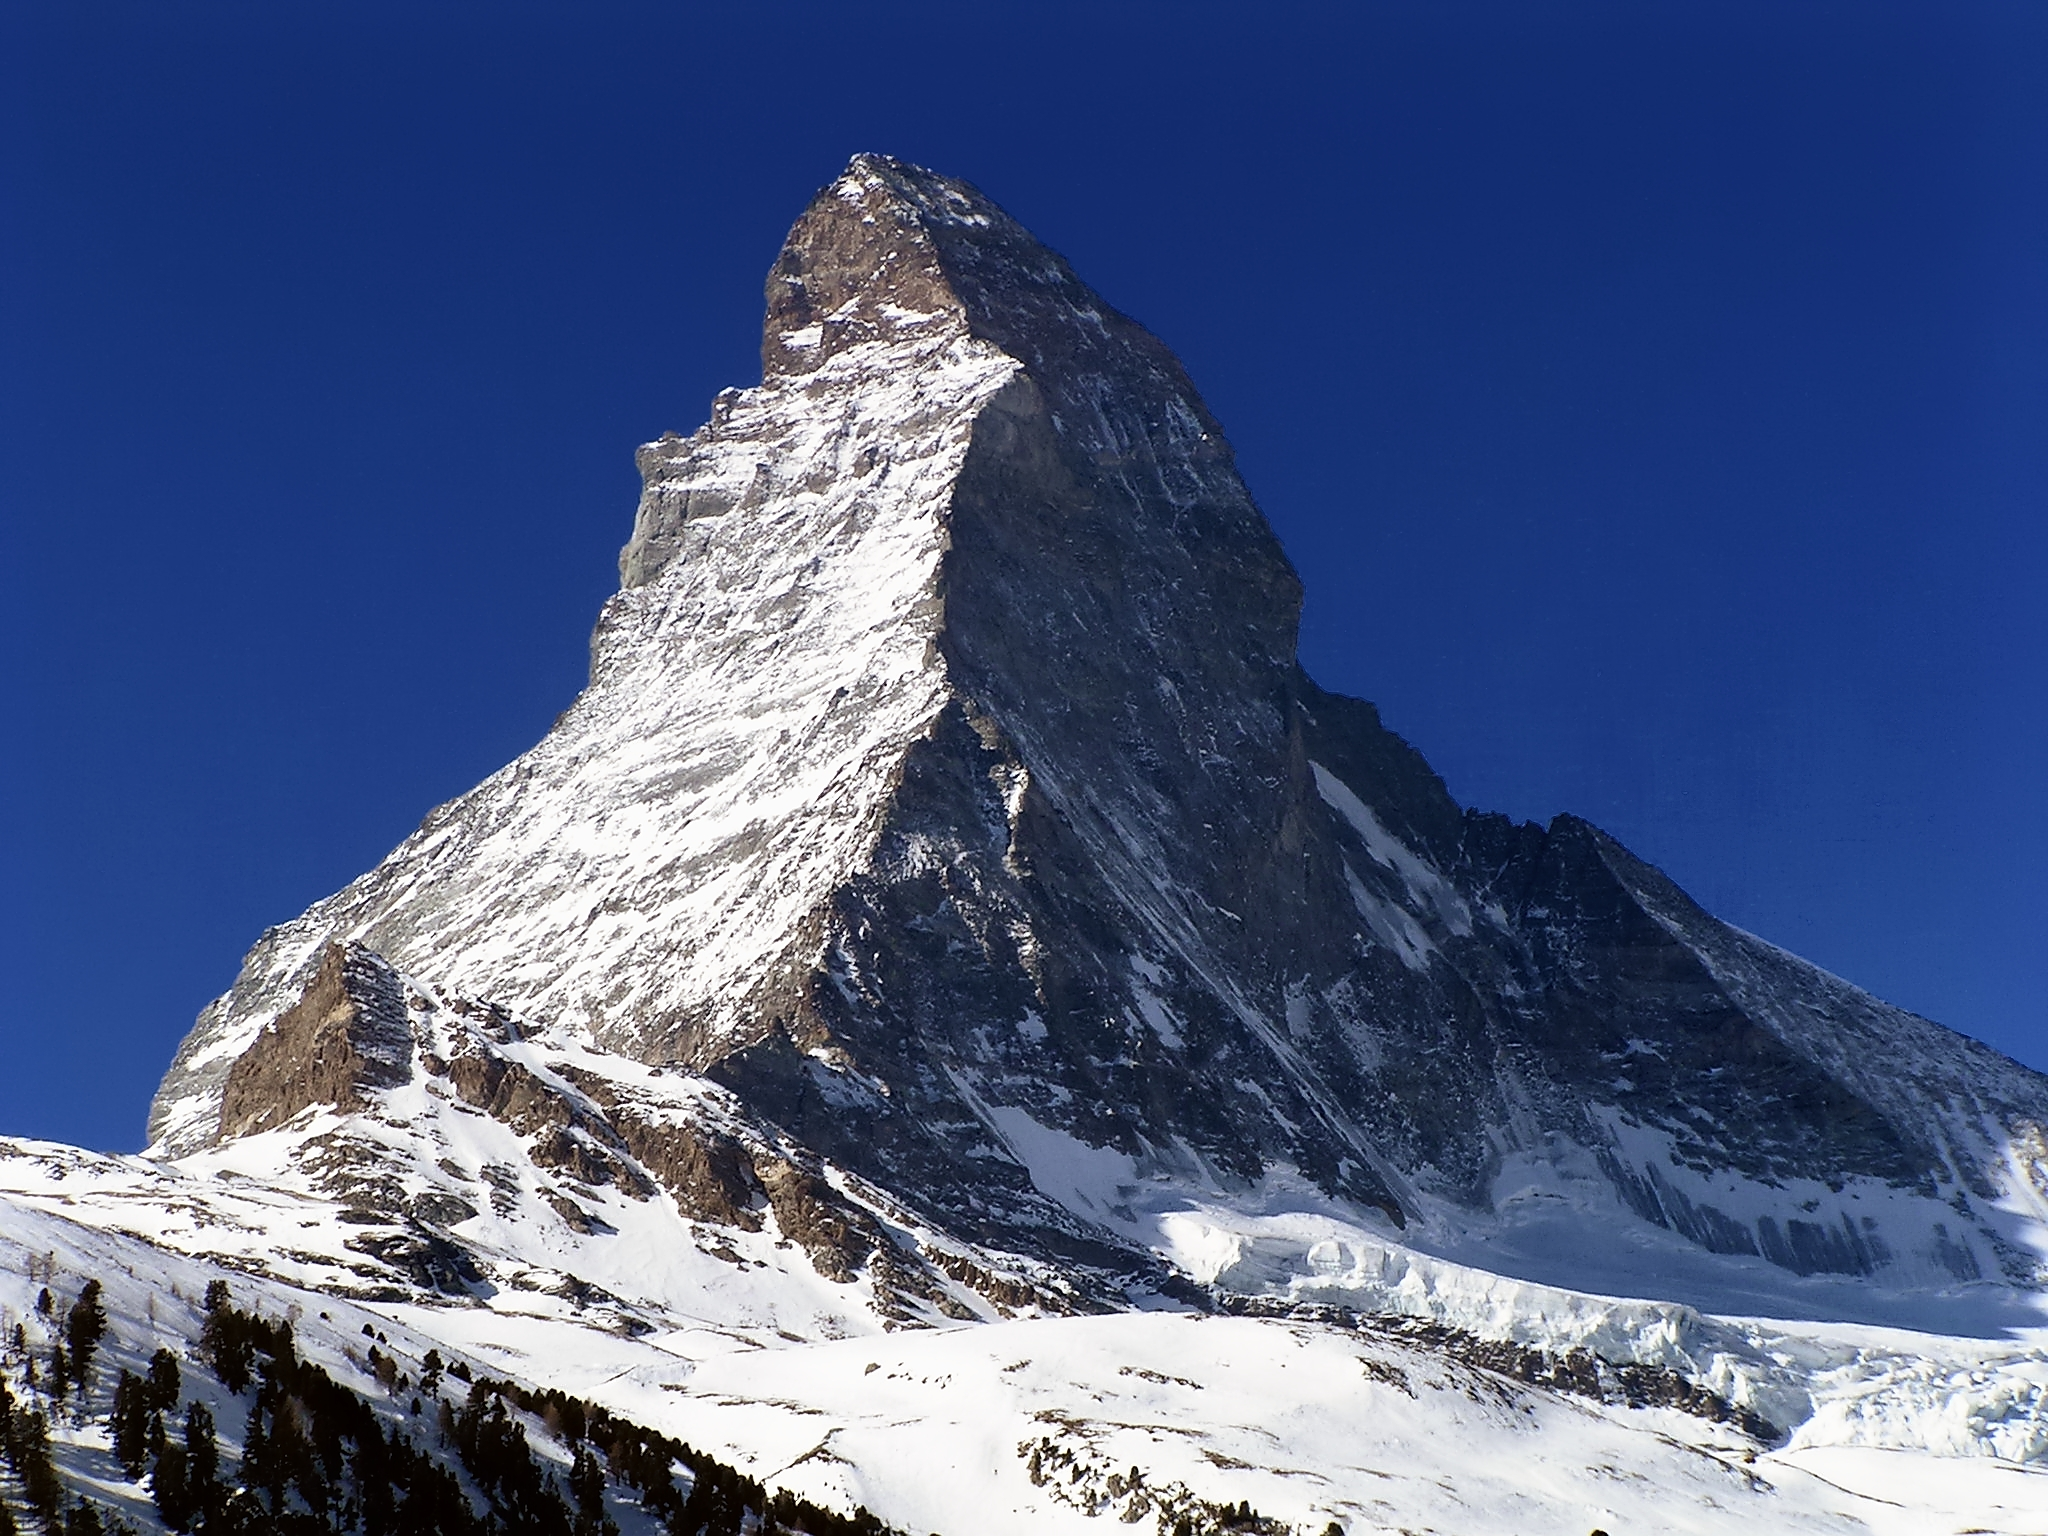
\includegraphics[width=0.9\paperwidth,trim=0cm 0cm 0cm 5cm]
  {Matterhorn-EastAndNorthside-viewedFromZermatt_landscapeformat-2}}}


\begin{document}
	
%\end{document}
\begin{frame}
  \begin{tikzpicture}[%remember picture,
  decoration={
  markings,
  %mark= at position 0cm with {\node{
\includegraphics[scale=0.2]{duck}};},
   mark= at position \fpeval{(\value{page})/200*22+1.8}cm 
    with {\node{
\includegraphics[scale=0.35,page=2]{duck}};},  
    mark= at position \fpeval{(\value{page})/200*22+1.2}cm 
    with {\node{
\includegraphics[scale=0.25]{duck}};},
  mark= at position \fpeval{(\value{page})/200*22+0.6}cm 
    with {\node{
\includegraphics[scale=0.25,page=2]{duck}};}, 
  mark= at position \fpeval{(\value{page})/200*22}cm 
    with {\node{
\includegraphics[scale=0.35]{duck}};}, 
  %mark= at position 22cm with {\node{
\includegraphics[scale=0.2]{duck}};}
  }
  ]
   \path[use as bounding box](0,0)rectangle(\textwidth,\textheight-15pt);  
   \path[%draw=red,thick,
   postaction=decorate] 
   (15,0.2) 
   --  (10.1,0.75)
   -- (9,1)
   -- (8,1)
   -- 
   (7,0.6)
   -- (6,1)
   -- (5,1.7)
   -- (4,2)
   -- (3,2.6)
   -- (2.1,3)
   -- (4,3.2)
   -- (5,3.8)
   -- (4,4.2)
   -- (6,5)
   -- (5,6)
   -- (6.4,6.8);
    
    % credit for background image
    \node[white,text width=.7\paperwidth,font=\tiny,align=center] at 
     ([yshift=0]current page.south) {Image source: \url{https://commons.wikimedia.org/wiki/File:Matterhorn-EastAndNorthside-viewedFromZermatt_landscapeformat-2.jpg}};  
    
  \end{tikzpicture}
  \pause[190]
\end{frame}	
	
\end{document}
